\documentclass[letterpaper,10pt]{article}

\usepackage{enumitem}
\usepackage{titling}
\usepackage{listings,listings-rust}
\usepackage{url}
\usepackage{soul}
\usepackage{hyperref}
\usepackage{setspace}
\usepackage{subfig}
\usepackage{sectsty}
\usepackage{pdfpages}
\usepackage{colortbl}
\usepackage{multirow}
\usepackage{multicol}
\usepackage{relsize}
\usepackage{amsmath}
\usepackage{wasysym}
\usepackage{fancyvrb}
\usepackage[yyyymmdd]{datetime}
\usepackage{amsmath,amssymb,amsthm,graphicx,xspace}
\usepackage[titlenotnumbered,noend,noline]{algorithm2e}
\usepackage[compact]{titlesec}
\usepackage{XCharter}
\usepackage[T1]{fontenc}
\usepackage[scaled]{beramono}
\usepackage[normalem]{ulem}
\usepackage{booktabs}
\usepackage{tikz}
\usetikzlibrary{arrows.meta,automata,shapes,trees,matrix,chains,scopes,positioning,calc,decorations.pathreplacing}
\tikzstyle{block} = [rectangle, draw, fill=blue!20, 
    text width=2.5em, text centered, rounded corners, minimum height=2em]
\tikzstyle{bw} = [rectangle, draw, fill=blue!20, 
    text width=4em, text centered, rounded corners, minimum height=2em]

\definecolor{namerow}{cmyk}{.40,.40,.40,.40}
\definecolor{namecol}{cmyk}{.40,.40,.40,.40}
\renewcommand{\dateseparator}{-}

\let\LaTeXtitle\title
\renewcommand{\title}[1]{\LaTeXtitle{\textsf{#1}}}

\lstset{basicstyle=\footnotesize\ttfamily,breaklines=true}

\newcommand{\CPP}{C\nolinebreak\hspace{-.05em}\raisebox{.4ex}{\tiny\bf +}\nolinebreak\hspace{-.10em}\raisebox{.4ex}{\tiny\bf +}}
\def\CPP{{C\nolinebreak[4]\hspace{-.05em}\raisebox{.4ex}{\tiny\bf ++}}}

\newcommand{\handout}[5]{
  \noindent
  \begin{center}
  \framebox{
    \vbox{
      \hbox to 5.78in { {\bf ECE459: Programming for Performance } \hfill #2 }
      \vspace{4mm}
      \hbox to 5.78in { {\Large \hfill #4  \hfill} }
      \vspace{2mm}
      \hbox to 5.78in { {\em #3 \hfill \today} }
    }
  }
  \end{center}
  \vspace*{4mm}
}

\newcommand{\lecture}[3]{\handout{#1}{#2}{#3}{Lecture #1}}
\newcommand{\tuple}[1]{\ensuremath{\left\langle #1 \right\rangle}\xspace}

\addtolength{\oddsidemargin}{-1.000in}
\addtolength{\evensidemargin}{-0.500in}
\addtolength{\textwidth}{2.0in}
\addtolength{\topmargin}{-1.000in}
\addtolength{\textheight}{1.75in}
\addtolength{\parskip}{\baselineskip}
\setlength{\parindent}{0in}
\renewcommand{\baselinestretch}{1.5}
\newcommand{\term}{Winter 2023}

\singlespace


\begin{document}

\lecture{28 --- Causal Profiling}{\term}{Jeff Zarnett}

\section*{Causal Profiling}
At this point we've got some experience in identifying areas of the program that we think are slow or are limiting the maximum performance of our program. If we are presented with more than one thing, how do we know which of those would yield the most benefit? Is it possible that optimizing something would actually have no effect or even a negative effect? The scientific approach would be to do an experiment and find out. That is, change the code, see the impact, re-evaluate. What causal profiling offers us is a way to run those experiments without changing any code. That could be a significant savings of time and effort. 

One such causal profiler is called Coz (pronounced like ``cause'')~\cite{coz}. It does a what-if analysis that says: what would be the impact of speeding up this particular part of the code? 

A very simple approach would just look at the time of the program and just calculate what happens if the runtime of function \texttt{work()} is reduced by, say, 10\%. But that isn't a realistic approach, because speeding up that function might have no overall impact or change the execution time by increasing lock contention or some other mechanism. No, we actually need a simulation. 

The key observation of the Coz profiler authors is the idea that speeding up some area of code is fundamentally the same as slowing down every other part of the code. It's all relative! This is what we would call a virtual speedup. How is the other code slowed down? Adding some pauses to (stopping the execution of) the other threads. That certainly makes them run slower. Maybe you're not convinced that slowing down everything else is equivalent?


Shown below is the argument from~\cite{coz} in visual form. The original runtime is shown as (a). Hypothetically, say we make function \texttt{f} faster by some factor $d = 40\%$ that gives us (b). But, if instead of actually making function \texttt{f} faster, let's pause other threads for $0.4 \times t(f)$ where $t(f)$ is the original execution time of \texttt{f}. Then we get an equivalent effect to that of optimizing \texttt{f} by $d$.
\begin{center}
	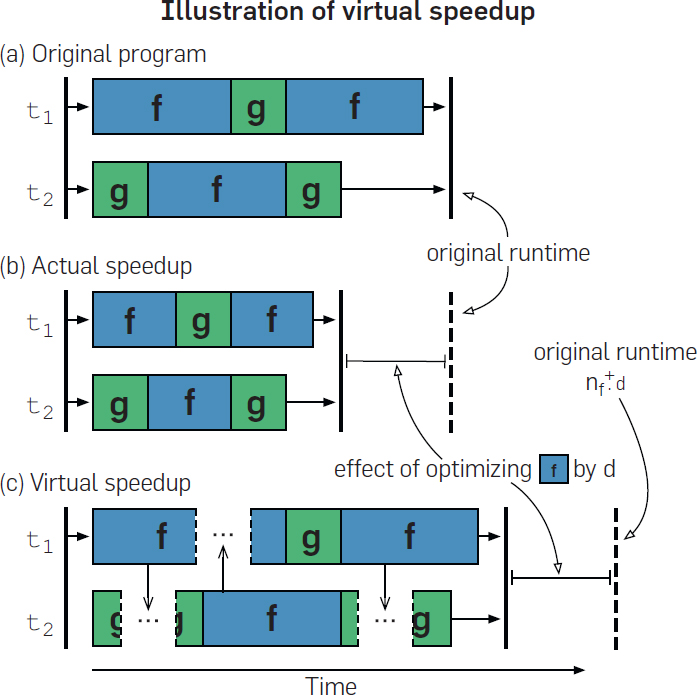
\includegraphics[width=0.4\textwidth]{images/virtual-speedup.jpg}
\end{center}

The tool provides some graphs of potential program speedup. From the recorded presentation, it might look something like the diagram below, where the boxes on the right correspond to different theoretical actions in the application being examined:

\begin{center}
	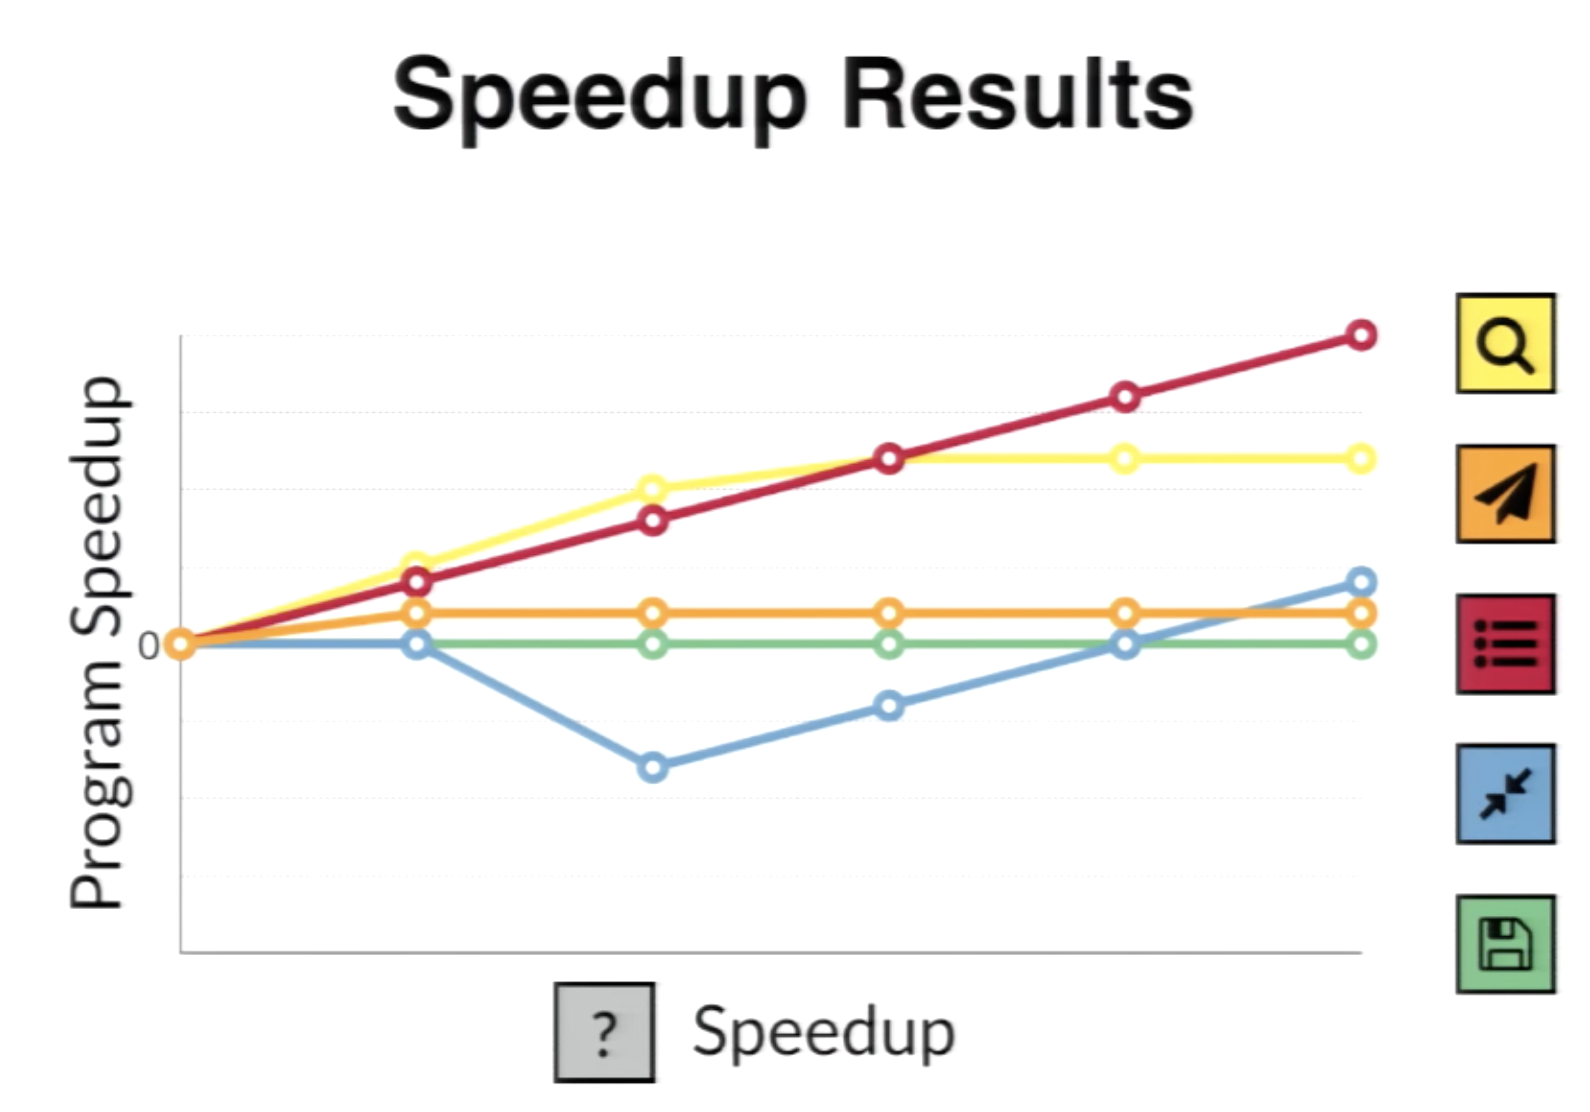
\includegraphics[width=0.4\textwidth]{images/coz-speedup-graph.png}
\end{center}

This pretend application shows all the possible outcomes, from continuous linear speedup, to speedup capped at some point, to no effect, and finally to where optimizing something makes the overall program runtime worse. 

It's easy to imagine scenarios corresponding to each of those. If we're computing the n-body problem, anything that improves the calculation of forces will certainly make things better. And it's easy to imagine that sometimes optimizing a part of the program does not improve anything because that code is not on the critical path. We can also easily imagine that improving something works up to a point where it ceases to be the limiting factor. But making things worse? We already covered that idea: speeding up a thread may increase lock contention or add something to the critical path. At some point, things may recover and be a net benefit.

It is important to remember that just because hypothetically speeding up a particular part of the program would be beneficial, doesn't mean that it's possible to speed up that part. And almost certainly not possible to do so to an arbitrary degree. We still have to make an assessment of what optimizations we can make and how difficult it would be to actually realize those improvements.

Once we've made a change to the program, then it's time to run an experiment again with the new baseline to see what else we can do.

The paper has a table summarizing the optimizations they applied to a few different programs, which seems to support the idea that the tool can be used effectively to get a meaningful speedup with relatively few lines of code~\cite{coz}:
\begin{center}
	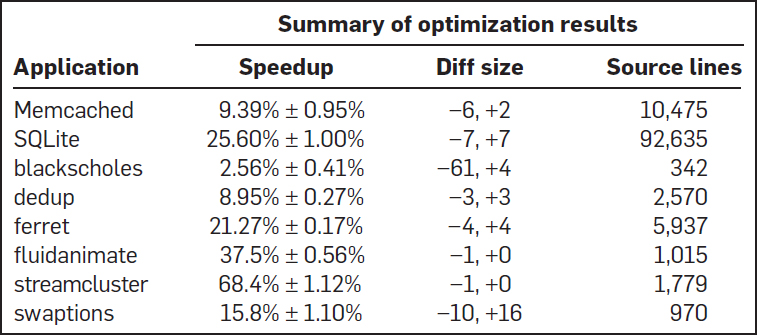
\includegraphics[width=0.6\textwidth]{images/coz-speedup.jpg}
\end{center}

There are potentially some limitations to this, of course. Putting pauses in the execution of the code can work when the execution of the program is all on the same machine and we have control over all the threads; it would need some meaningful extension to work for a distributed system where coordinating things across many servers would be needed.

Using some benchmarking workload, the authors estimate a 17.6\% overhead for this tool, which is broken down into 2.6\% for startup debug information collection, sampling at 4.8\%, and 10.2\% is the delay that's caused by slowing down other threads to create a virtual speedup~\cite{coz}.

If you'd like to see some more details of the tool, you can see the author presentation at the ACM symposium here: \url{https://www.youtube.com/watch?v=jE0V-p1odPg}

\subsection*{The Next Generation: SCOZ}
A few years later, another group of researchers worked to extend the Coz profiler to account for some limitations: inability to look at multi-process applications (which we just talked about), but also cases where the OS itself becomes a bottleneck~\cite{scoz}. You may recall that looking into the kernel is not always permitted for a given profiling tool -- depending on permissions.  It is therefore obvious to imagine that if one cannot look, then one cannot touch. 

If, indeed, the kernel is a bottleneck, it may or may not be possible to do very much about it. Avoiding system calls is one of the ``do less work'' strategies that you have likely already considered; oftentimes doing the system call is because we must. In an open-source OS or a kernel module we control, then we would have the ability to do something about it, if coz could give some recommendations.

The approach of~\cite{scoz} is to move from a thread-based system to a core-based one. So where, previously, to simulate speedup of a particular section of code the tool would pause all other threads, now it pauses execution on all other cores. There are some details to consider about what to do when there are idle cores to make sure that the delay is charged to the ``right'' core when one is woken up by another. The diagram the authors provides helps to explain it well:

\begin{center}
	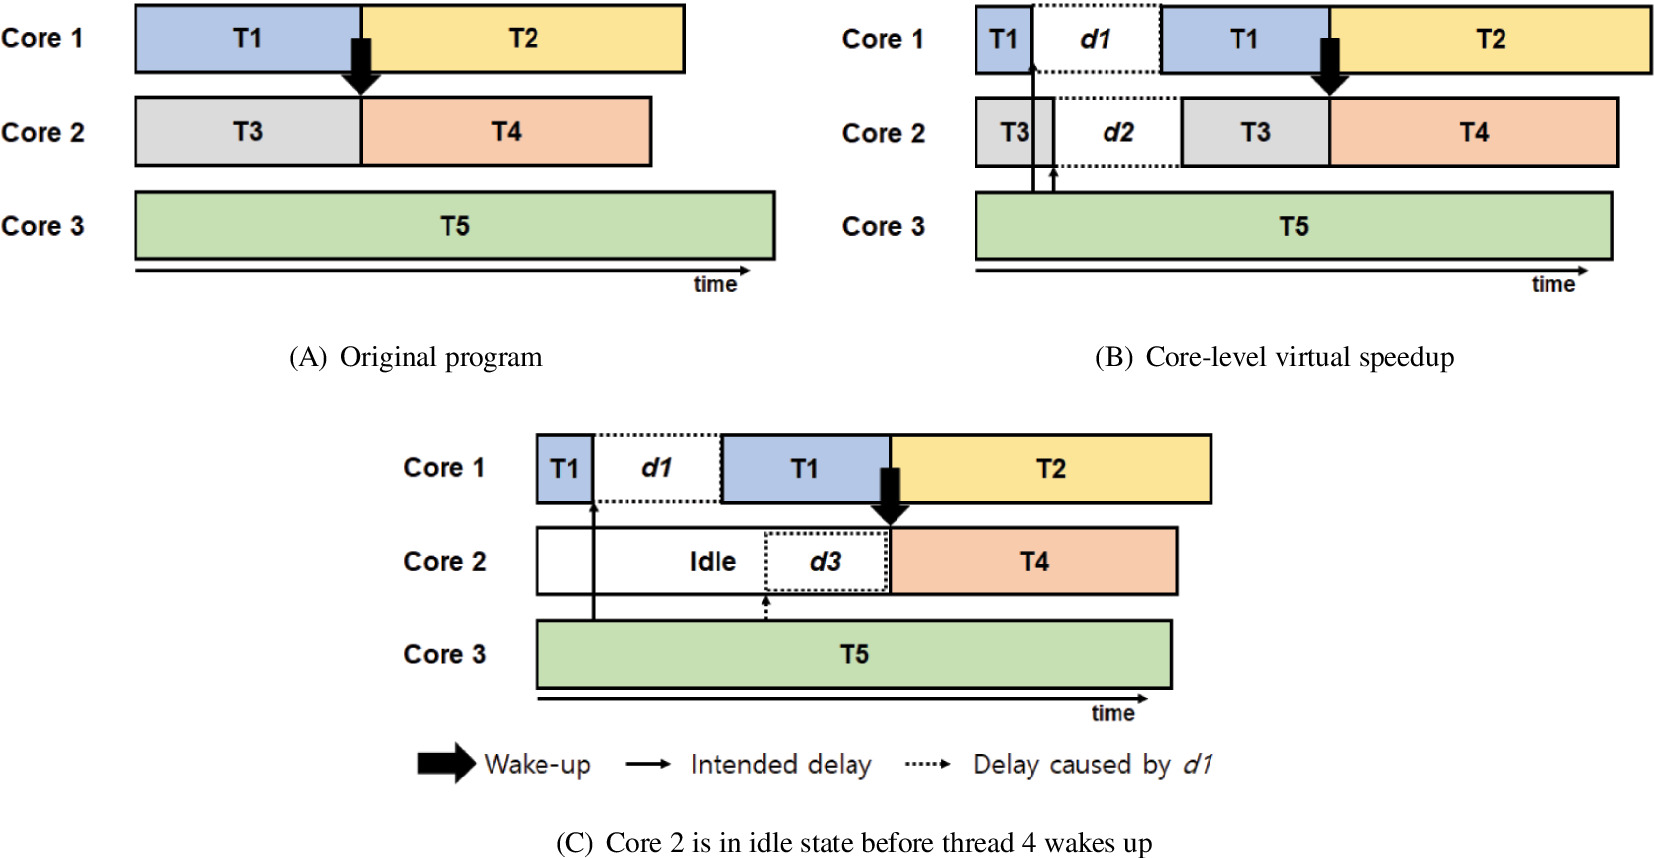
\includegraphics[width=0.8\textwidth]{images/scoz-delay.jpg}
\end{center}

The implementation involves one profiler thread for each core to manage its behaviour. The thread is pinned to the core, and its purpose is primarily to call the \texttt{ndelay} interface (with preemption temporarily disabled) to stop execution of code on that specific core~\cite{scoz}. 

This extension does allow scoz to do more than coz, but it does require running within the kernel, which imposes certain limitations to where and how it can be applied. That's an interesting tradeoff!

\input{bibliography.tex}

\end{document}
